
%\section{Overview of the Silicon Tracking System (STS)}
All semiconductor-based detector systems include very similar functions. The signals from the detector channels have to be amplified and processed for storage and analysis. The sensor, analog-digital converter, and all the necessary support structures, and data  are often referred to as a detector module. Apart from these structures, there are also services and design constraints that need to be taken into account while designing a detector. One of the first decisions is the detector material, which depends on many factors like the availability, energy needed for electron-hole production, technological feasibility, or integration with the electronics. Silicon (Si), germanium (Ge), gallium arsenide (GaAs) and Diamond are the most common semiconductor detector materials used~\cite{Lutz:1999wg,Hartmann:2017gzy}.


This chapter aims to present an introduction to silicon-based detector systems and general working principles. Subsequently, the design of the \gls{STS} is discussed with a focus on the hardware. Finally, the requirements for the detector control system are considered. 

\section{Fundamentals of the silicon detector}
Semiconductors can be considered ionization chambers, which feature a pair of electrodes and applied external voltage. The particles passing through the volume of a sensor lose their energy-producing electron and hole pair. The deposited charge is retrieved by one or more electrodes. The analog signals are converted into digital ones, processed, and analyzed.

To achieve precise particle position the electrodes can be segmented into strips. To address this problem, the electrodes can be segmented into strips. Figure~\ref{fig_si} shows an example of implementing segmented electrodes to determine the particle position. To achieve the two-dimensional information, the second electrode strips have usually an inclination of a few degrees. Hence, the contribution of fake ghost hits is minimized.  

\begin{figure}[!h]
\centering
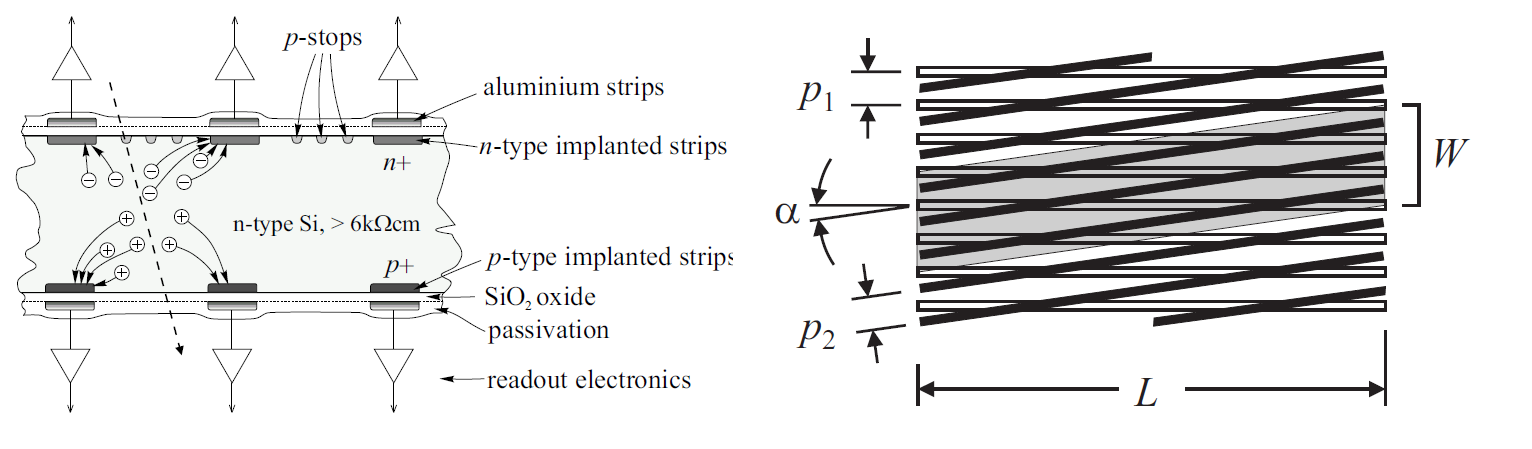
\includegraphics[width=0.95\columnwidth]{Chapter2/images/silicons.png}
\caption{The segmented electrode enables defining the particle position (left)~\cite{Sokolov:2006vdx}. The right scheme depicts the strips oriented at a small angle $\alpha$, which aims to reduce fake hits~\cite{Spieler}.}
\label{fig_si}
\end{figure}
\newpage

The operation principle of semiconductor-based devices is related to the fact that the charged particles traversing the volume of the detector may ionize it. %The mean value of the energy loss in the medium is given by the Bethe-Bloch formula:
%\begin{equation}
%-\dfrac{\mathrm dE}{\mathrm dx} = 4 \pi N_{a} r_{e}^{2} m_{e} c^{2} z^{2}  \dfrac{Z}{A} \frac{1}{\beta^{2}} \left[ \frac{1}{2}\ln(\frac{2m_{e}\gamma^{2}c^{2} T_{max}}{I^{2}}) - \beta^{2} -  \frac{\delta(\gamma)}{Z}\right]
%\end{equation}
%Where z is the charge of the particle, $T_{max}$ is the maximum kinetic energy that can be transferred to a free electron in a single collision, I is the mean excitation energy, Z the atomic number, A the atomic mass, $N_{A}$ the Avogadro’s number, $m_{e}$ the electron mass, c the speed of light, $r_{e}$ the classical electron radius, $\beta = v/c$ and $\gamma = \frac{1}{\sqrt{1-\beta^{2}}}$ and $\delta$ density effect correction. 
On the other hand, photons must first interact with an electron through the photo or Compton effect, or with the Si nucleus. 

The sensitive volume of a silicon sensor produces an average signal current given by 
\begin{equation}
    Q_{s} = \frac{E}{E_{i}}e
\end{equation}
where E is the absorbed energy, $E_{i}$ is the energy required to form a charge pair. The energy needs to be greater than the band gap of the semiconductor so that the electron can move to the conduction band. The silicon has a gap of \SI{1.12}{\eV}. Nevertheless, the commonly used ionization energy for silicon is about \SI{3.6}{\eV}. This effect is related to the fact that only about 30\% of the particle energy is converted into an electrical signal, and the rest goes into phonon excitation (lattice vibrations). A typical charge deposition by a minimum ionizing particle in a \SI{300}{\micro\metre} thick wafer is around 25000 electron-hole pairs.

Considering a simple example if a sensor had about $\sim10^{9}$ thermally produced free charge carriers\footnote{Electrons or holes introduced to the conduction (valence) band by doping.}, but a passing charged particle would generate only $\sim2\times10^{4}$ electrons-hole pairs. Such a signal would be lost in the remaining free-charge carriers. There are two ways to address this problem, either by cooling the sensor to very low temperatures or depleting the silicon volume of free-charge carriers. The depletion process of a pn-junction requires applying an external voltage so that the sensor is fully depleted~\cite{Spieler}. This external voltage $V$ disturbs the equilibrium of spontaneous generation and recombination of electrons/holes. It increases the potential barrier of the pn-junction and the depletion width. 

The full depletion voltage is one of the most important parameters for silicon sensors, as it defines the operating range. 
\begin{equation}
    V_{FD} = \frac{D^{2}}{2\epsilon \mu \rho},
\end{equation}
where D is the sensor thickness, $\epsilon$ is the dielectric constant, $\mu$ is the mobility and $\rho$ the resistivity.

When the sensor is operated in the over-depleted mode, the electric field is established.
\begin{equation}
    E_{max/min} = \frac{V_{bias}\pm V_{FD}}{D}
\end{equation}
where $V_{FD}$ is the effective full depletion voltage and $V_{bias}$ is the additional voltage. The thermally generated electron-hole pairs are swept out of the depletion region. This effect results in a reverse current called leakage current which is strongly influenced by mid-gap levels occupied by impurities. The current increases linearly with the $\sqrt{V}$ until the detector reaches full depletion. An electric breakdown is found at greater bias voltages, where the current begins to increase exponentially. The breakdown can be understood by either "avalanche breakdown" (charge multiplication in collisions with the lattice) or "Zener breakdown" (based on the quantum mechanical "tunnel effect")~\cite{Hartmann:2017gzy}.

If the detector is fully depleted, the generated electrons and holes drift in the electric field according to their velocities $\nu_{p}$ and $\nu_{n}$ in the direction of respective electrodes. The current induced by a single charge carrier can be described by Ramo's theorem:
\begin{equation}
    I = q_{0}\frac{v_{n,p}}{D}
\end{equation}
where the drift velocity depends on the mobility of the holes and electrons and the electric field strength, and d is the thickness.

\section{Radiation damage to the silicon sensors}
\label{silicon_damage}
% Annealing after radiation damage
To understand the properties of the silicon sensor after irradiation, it is necessary to consider the damage done to the lattice by the particles and the process called annealing. Radiation damage can be divided into two main groups: displacement damage and ionization damage. The first mentioned phenomenon is related to the incident particles displacing the silicon atoms from their position in the lattice. The ionization damage occurs in the insulating layers of the sensor (usually forming $\mathrm{SiO_{2}-Si}$ interface states~\cite{Moll:1999kv}. Displaced atoms form defects, which introduce new levels in the band gap, therefore changing the properties of the semiconductor. It results in the increase of the dark current, change of depletion voltage, and decrease of Charge Collection Efficiency (\gls{CCE}). In practice, the damage depends on the particle interacting with the sensors and its energy. Figure~\ref{fig_niel_si} describes the behavior of displacement damage for different particles and their energies.  
\begin{figure}[!h]
\centering
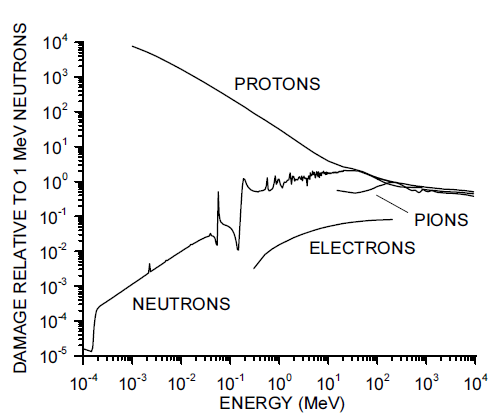
\includegraphics[width=0.7\columnwidth]{Chapter2/images/displacement_damage.png}
\caption{Displacement damage vs. energy for neutrons, protons, pions, and electrons,
plotted relative to 1\,MeV neutrons~\cite{Spieler}.}
\label{fig_niel_si}
\end{figure}

Annealing can be described as the combination of various effects, such as the movement of particles or defects through the lattice structure, the rearrangement, or break-up of defects, and the interaction between defects as they propagate. Silicon sensors annealing is a process used to reduce the amount of leakage current present in silicon sensors. This process involves heating the sensors to a very high temperature for an extended period of time, allowing the bonds between the atoms in the silicon lattice to become more stable and reduce the amount of current flowing through the device. The annealing process also helps to reduce the amount of noise generated by the sensor, as well as improve its temperature stability. \bigbreak

\textbf{Leakage current}\bigbreak
Production of additional mid-gap levels is the major contributor to the increase of leakage current during the radiation. It was also found in a number of experiments that the sensor leakage current is related to the fluence as follows:

\begin{equation}
\label{eq:fluence}
    I_{d} = I_{0} + \alpha \phi Ad
\end{equation}
where $I_{0}$ is the leakage current before the irradiation, $\alpha$ is a damage coefficient dependent on particle type and temperature, $\phi$ is the particle fluence, d is the detector thickness, and A is the area. Figure~\ref{fig_leakage_theory} provides a more detailed overview of damage-induced bulk current in different types of silicon detectors. Moreover, leakage current changes also with the temperature:
\begin{equation}
\label{Sil:temp}
    I(T) \propto T^{2}e^{\frac{-E}{2kT}}
\end{equation}
If the temperature of the silicon sensors is known, then it is possible to normalize the leakage current to a predefined value (e.g., \SI{20}{\celsius}). It allows for comparing the leakage current of sensors before and after irradiation, even though the ambient conditions were different. 

It allows us to scale down leakage current to $20\,^{\circ}$C using the equation \ref{Sil:scal}.
 
\begin{equation}
\label{Sil:scal}
    \frac{I_{R}(T_{2})}{I_{R}(T_{1})} = (\frac{T_{2}}{T_{1}})^{2}e^{\frac{-E_{g}}{2kT}(\frac{T_{1}-T_{2}}{T_{1}T_{2}})}
\end{equation}
where $E_{g}$ is the band gap, k is the Boltzmann constant, I is the current and T is the temperature.
%\begin{figure}[!h]
%\centering
%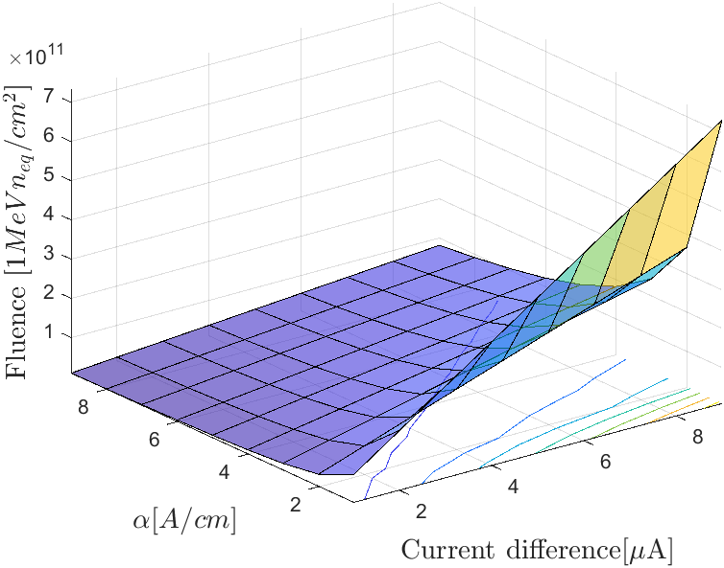
\includegraphics[width=0.65\columnwidth]{Chapter2/images/Leakage_current.png}
%\caption{Fluence estimations based on Equation~\ref{eq:fluence} for the typical leakage %changes during the \gls{mCBM} experiment.}
%\label{fig_leakage}
%\end{figure}
% Explain the graph a little bit different

\begin{figure}[!h]
\centering
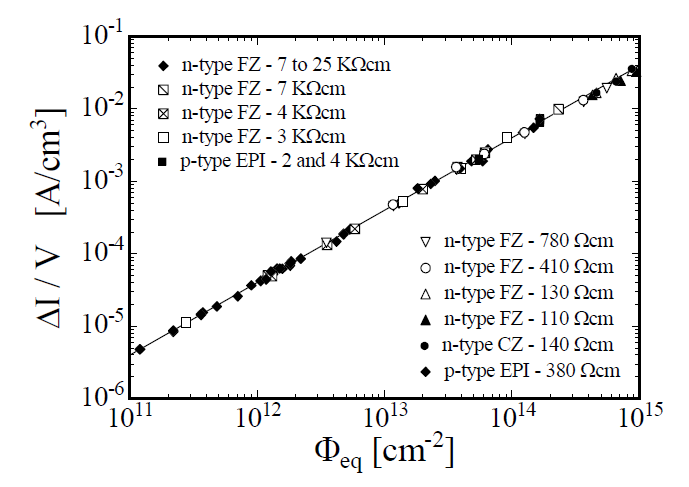
\includegraphics[width=0.75\columnwidth]{Chapter2/images/lekage_current_fluence.png}
\caption{Damage induced bulk current as a function of particle fluence
for different detector types~\cite{Moll:1999kv}.}
\label{fig_leakage_theory}
\end{figure}
% Information about the sensors used in the upper one
\textbf{Depletion Voltage}\bigbreak

Defects caused by radiation increase the leakage current of the device and thus reduce the depletion voltage. In addition, the radiation can cause the charge carriers to become trapped, reducing the mobility of the carriers and further reducing the depletion voltage. For an n-type-doped silicon sensor, the effects of radiation on the depletion voltage are more pronounced compared to a p-type-doped sensor, as the majority of carriers in an n-type-doped sensor are electrons, which are more easily affected by radiation than holes.  \bigbreak

\textbf{Signal-to-noise ratio and Charge Collection Efficiency }\bigbreak
Signal-to-noise ratio and CCE are two very important factors characterizing the detector. The noise level can be controlled by operating the detector at low temperatures or by limiting the exposition to electromagnetic interference. On the other hand, the CCE of non-irradiated sensors is assumed to be 100\%. The CCE after the irradiation could be defined as the ratio:

\begin{equation}
    \eta = 100\%\times\frac{Q_{irr}}{Q}
\end{equation}
where $Q_{irr}$ is the charge collected by the irradiated sensor, and $Q$ is the charge collected by non-irradiated sensor. 
The CCE depends on the depletion voltage and its changes with the radiation, as the full collection of the charge could only be achieved at the maximum electric field. Therefore, the fluence and/or depletion voltage remain crucial for the operation of the detector. 

\section{Design of the Silicon Tracking System}
\label{STS}

The physics observables together with the foreseen accelerator energy and beam intensity mentioned in the previous chapter define the requirements for the detector system. The \gls{STS} is designed to provide track reconstruction and momentum determination of the charged particles. Those particles are produced in collisions of an ion beam with energies from \agev{2} to \agev{14} (protons \gev{29}) with a target. For example, a central Au+Au collision results in up to 700 tracks. The \gls{STS} extends more than \SI{1}{\metre} downstream of the target and will be installed in a volume of \SI{3}{\cubic\metre}. 
% on average 700 tracks, change the sentence anyway

In order to achieve physics goals, \gls{STS} has to address the following:
\begin{itemize}
    \item  aperture - the aperture of the whole experiment is assumed to cover polar angles from \SI{2}{\degree} up to \SI{25}{\degree}. This range corresponds to center-of-mass rapidity close to the beam rapidity. 
    \item spatial resolution - a single-hit resolution of about \SI{20}{\micro\metre} in X direction and \SI{120}{\micro\metre} in Y, 
    \item single-hit efficiency - the detector layer should provide almost 100\% detection efficiency. The signal-to-noise\footnote{Ratio of the most probable signal amplitude for a minimum ionizing particle divided by the root mean square of the single strip noise.} ratio needs to be over 10. Having that, the track reconstruction efficiency should exceed 95\% for particle momenta larger than \agevc{1}. 
    \item momentum resolution - it is mainly influenced by the material budget of the system. The \gls{STS} is designed with the aim to avoid excessive multiple scattering. It is achieved by placing the electronics, mechanical infrastructure and cooling outside the active area. For the \gls{STS} the momentum resolution of $\Delta p/p = 1.8\%$ is required. 
    \item radiation hardness - the silicon sensors and the electronics need to withstand the total dose of $10^{14}\,\mathrm{neutrons/cm^{2}~(1\,MeV eq)}$. It was confirmed that after receiving twice the mentioned dose the CCE decreases by up to 20\%. The fluence of \kgy{12} is expected only for the 5 - 10\% sensors in the innermost region of the detector after 10 years of operation, 2 months per year of \agev{10} Au+Au collisions at \mhz{10} interaction rate~\cite{Heuser:54798}.
    \item hit rates and readout - the hit rates of charged particles for the inner-most silicon sensors (\mhz{10} per $\mathrm{cm^{2}}$ define the requirements for the readout system (signal shaping time, number of readout channels etc.)
\end{itemize}


\begin{figure}[!h]
\centering
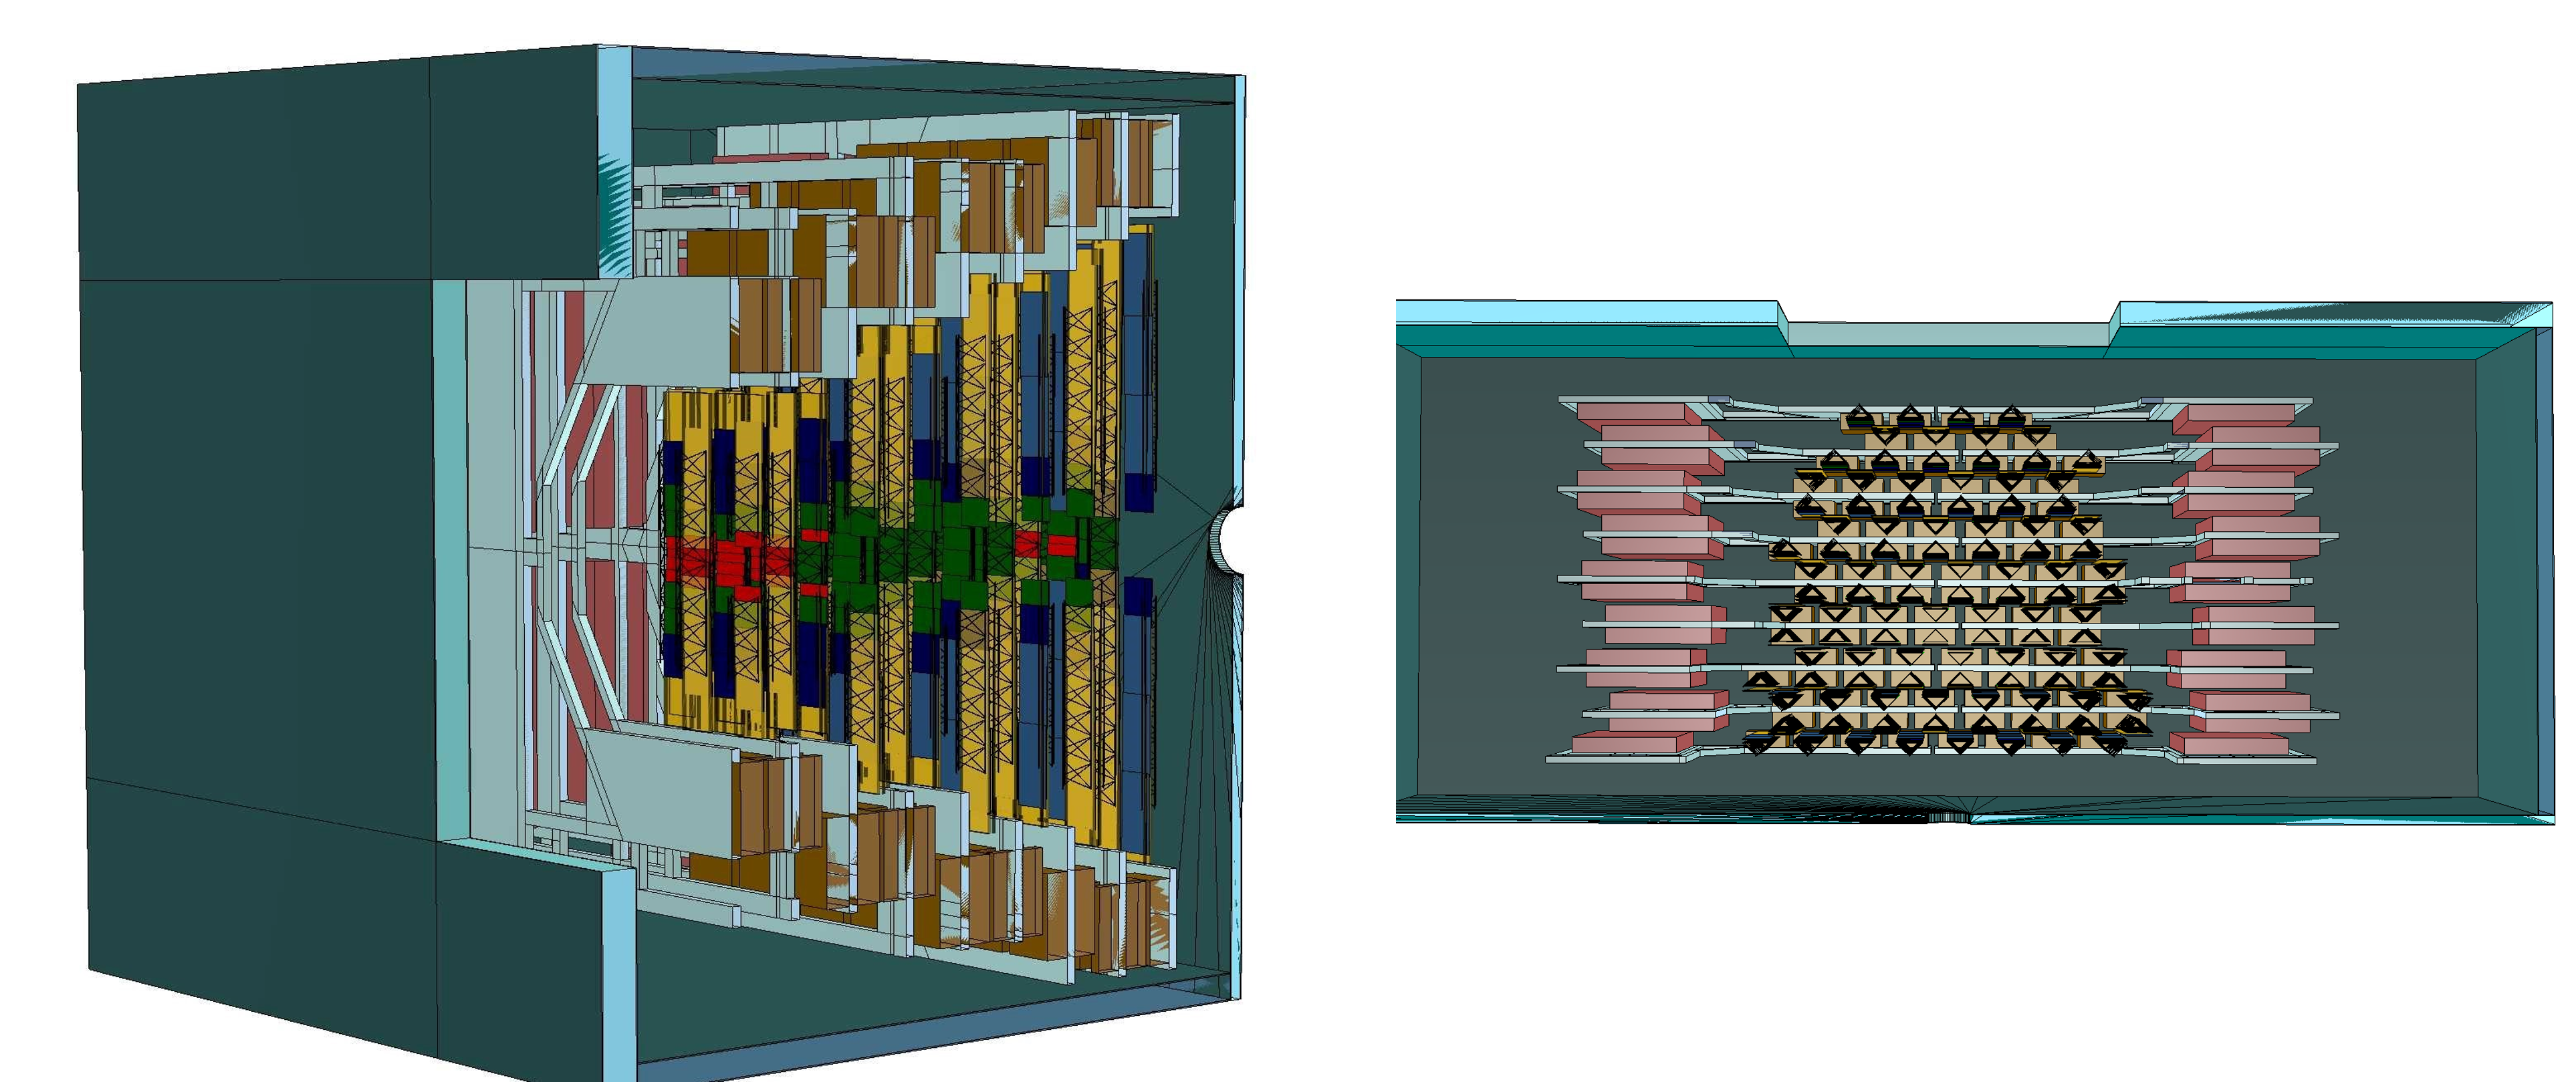
\includegraphics[width=0.85\columnwidth]{Chapter2/images/STS.png}
\caption{A simplified geometry of the Silicon Tracking System. The 8 tracking stations cover the polar angle from \SI{2}{\degree} up to \SI{25}{\degree}.}
\label{fig_STS}
\end{figure}
A simplified CAD drawing of the \gls{STS} is presented in Figure~\ref{fig_STS}. The detector consists of 876 detectors modules. A module is composed of a double-sided silicon microstrip sensor, ultralight microcables (of up to \SI{50}{\centi\metre} length) and Front End Boards (\gls{FEB}) populated with Application-specific integrated circuit (\glspl{ASIC}) glued to T-shaped aluminum structures (so-called fins). The modules are mounted on carbon fiber support structures that populate C-frames~\cite{progress_report_2016}. Two C-frames form a tracking station of \gls{STS}.  Figure~\ref{fig_assembly} depicts a simplified assembly workflow of \gls{STS}.
The modules are produced in 166 variants, which differ in sensor size, micro-cable length, and the orientation of the Front End Electronics~(\gls{FEE}).  


The stations are placed inside a thermally insulated box that resides in a dipole magnet gap. During \gls{STS} operation, the temperature inside the enclosure will be gradually decreased with the increasing radiation damage to the silicon sensors, to minimize thermal runaway~\cite{Spieler}. The largest amount of heat is dissipated by the low-voltage powering of the electronics and not the sensors themselves. Hence, effective cooling is needed to address this problem.
The temperature of about \SI{-10}{\celsius} will ensure a safe performance (away from the thermal runaway\footnote{Thermal runaway occurs when the power dissipation of a device increases rapidly with temperature, and it is impossible to evacuate the excess heat.} temperatures) of the semiconductor sensors and minimize the contribution of the shot noise~\cite{Spieler}. The low ambient temperature also sets hard limits on the frost point inside the STS enclosure. As the coolant temperatures might reach down to \SI{-40}{\celsius}, the frost point needs to be below \SI{-45}{\celsius} at all times. 

\newpage
\begin{figure}[!h]
\centering
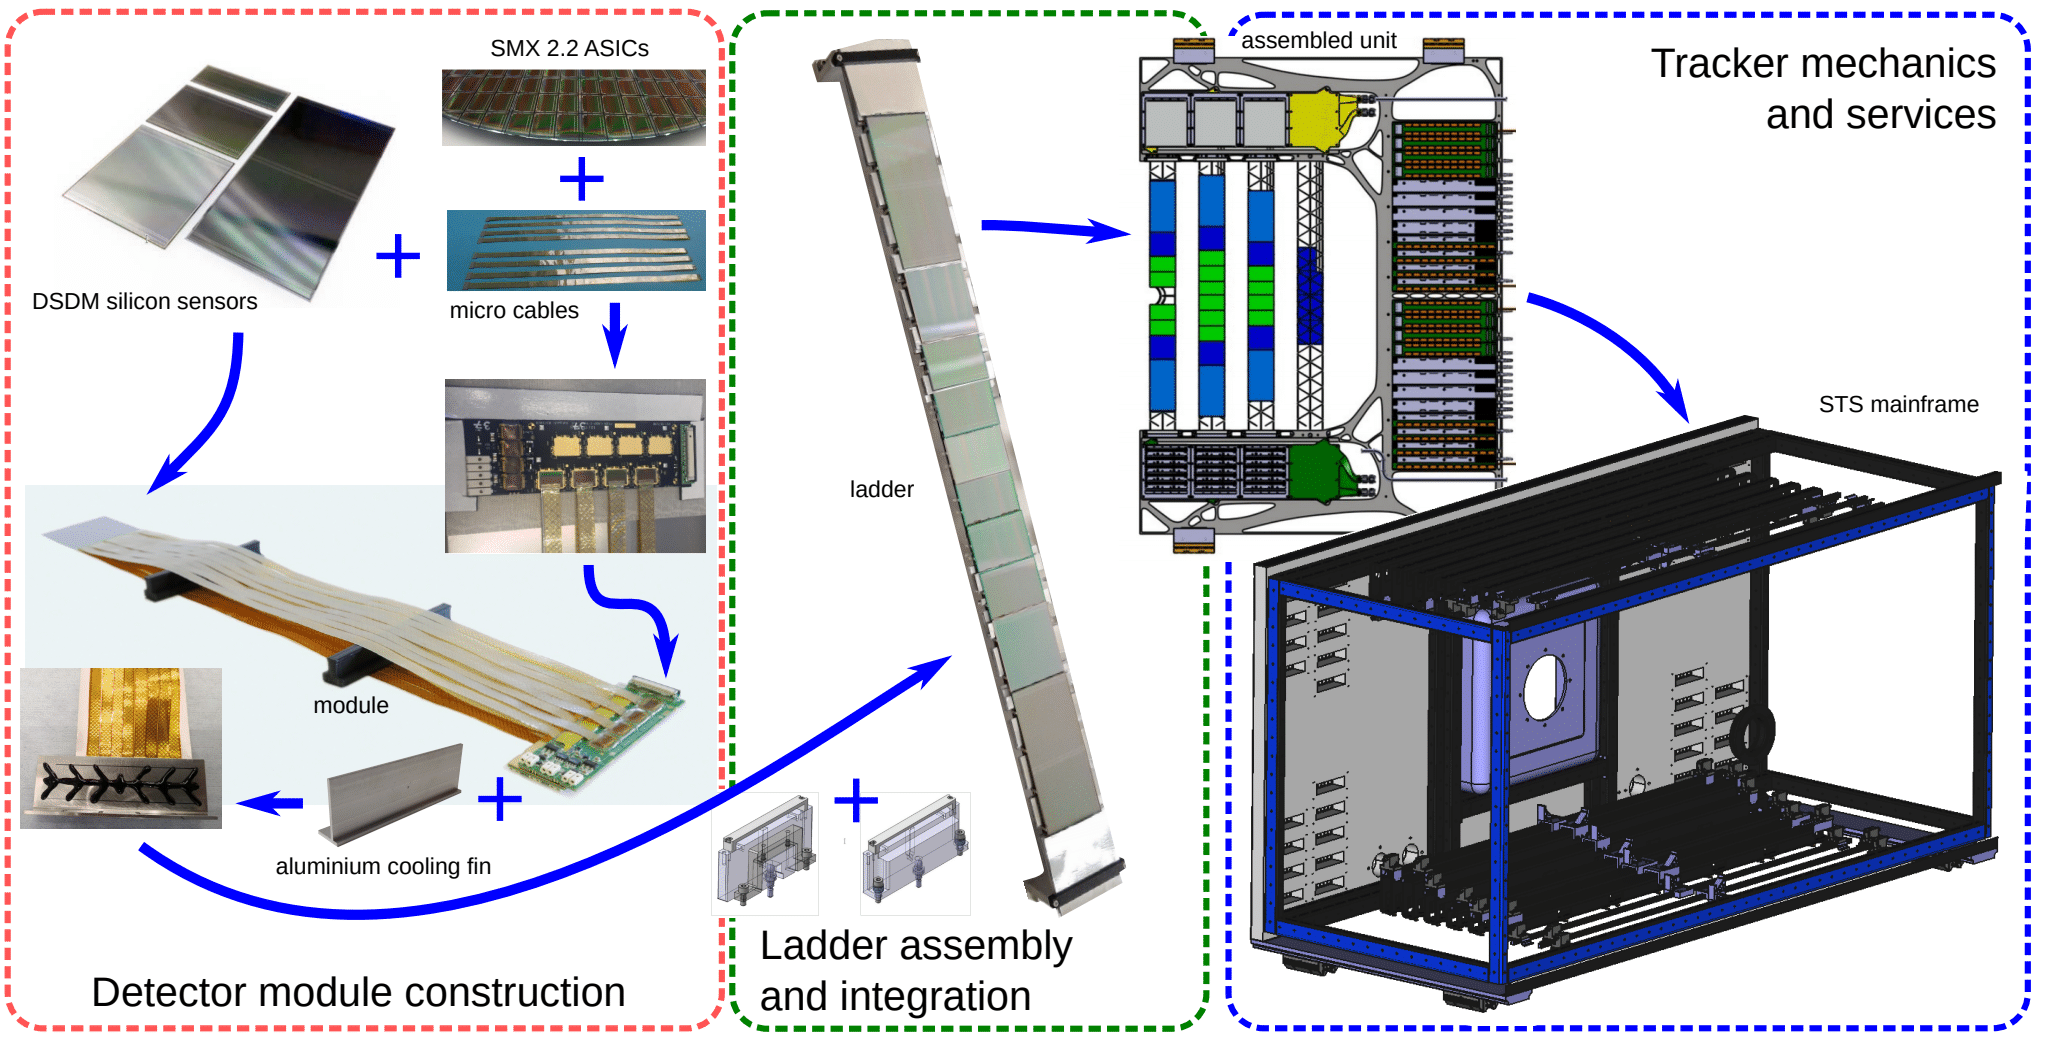
\includegraphics[width=1\columnwidth]{Chapter2/images/assembly_sequence.png}
\caption{A simplified assembly workflow of the \gls{STS}; silicon sensors are connected to the ASICs on the \glspl{FEB} via microcables, then the modules are assembled onto carbon fiber ladders which form a C-frame~\cite{Teklishyn}.}
\label{fig_assembly}
\end{figure}

%The evolution of different experimental setups constructed for the purpose of testing components of the \gls{STS} is depicted in Figure \ref{fig_evolution_STS}. 

%\begin{figure}[!h]
%\centering
%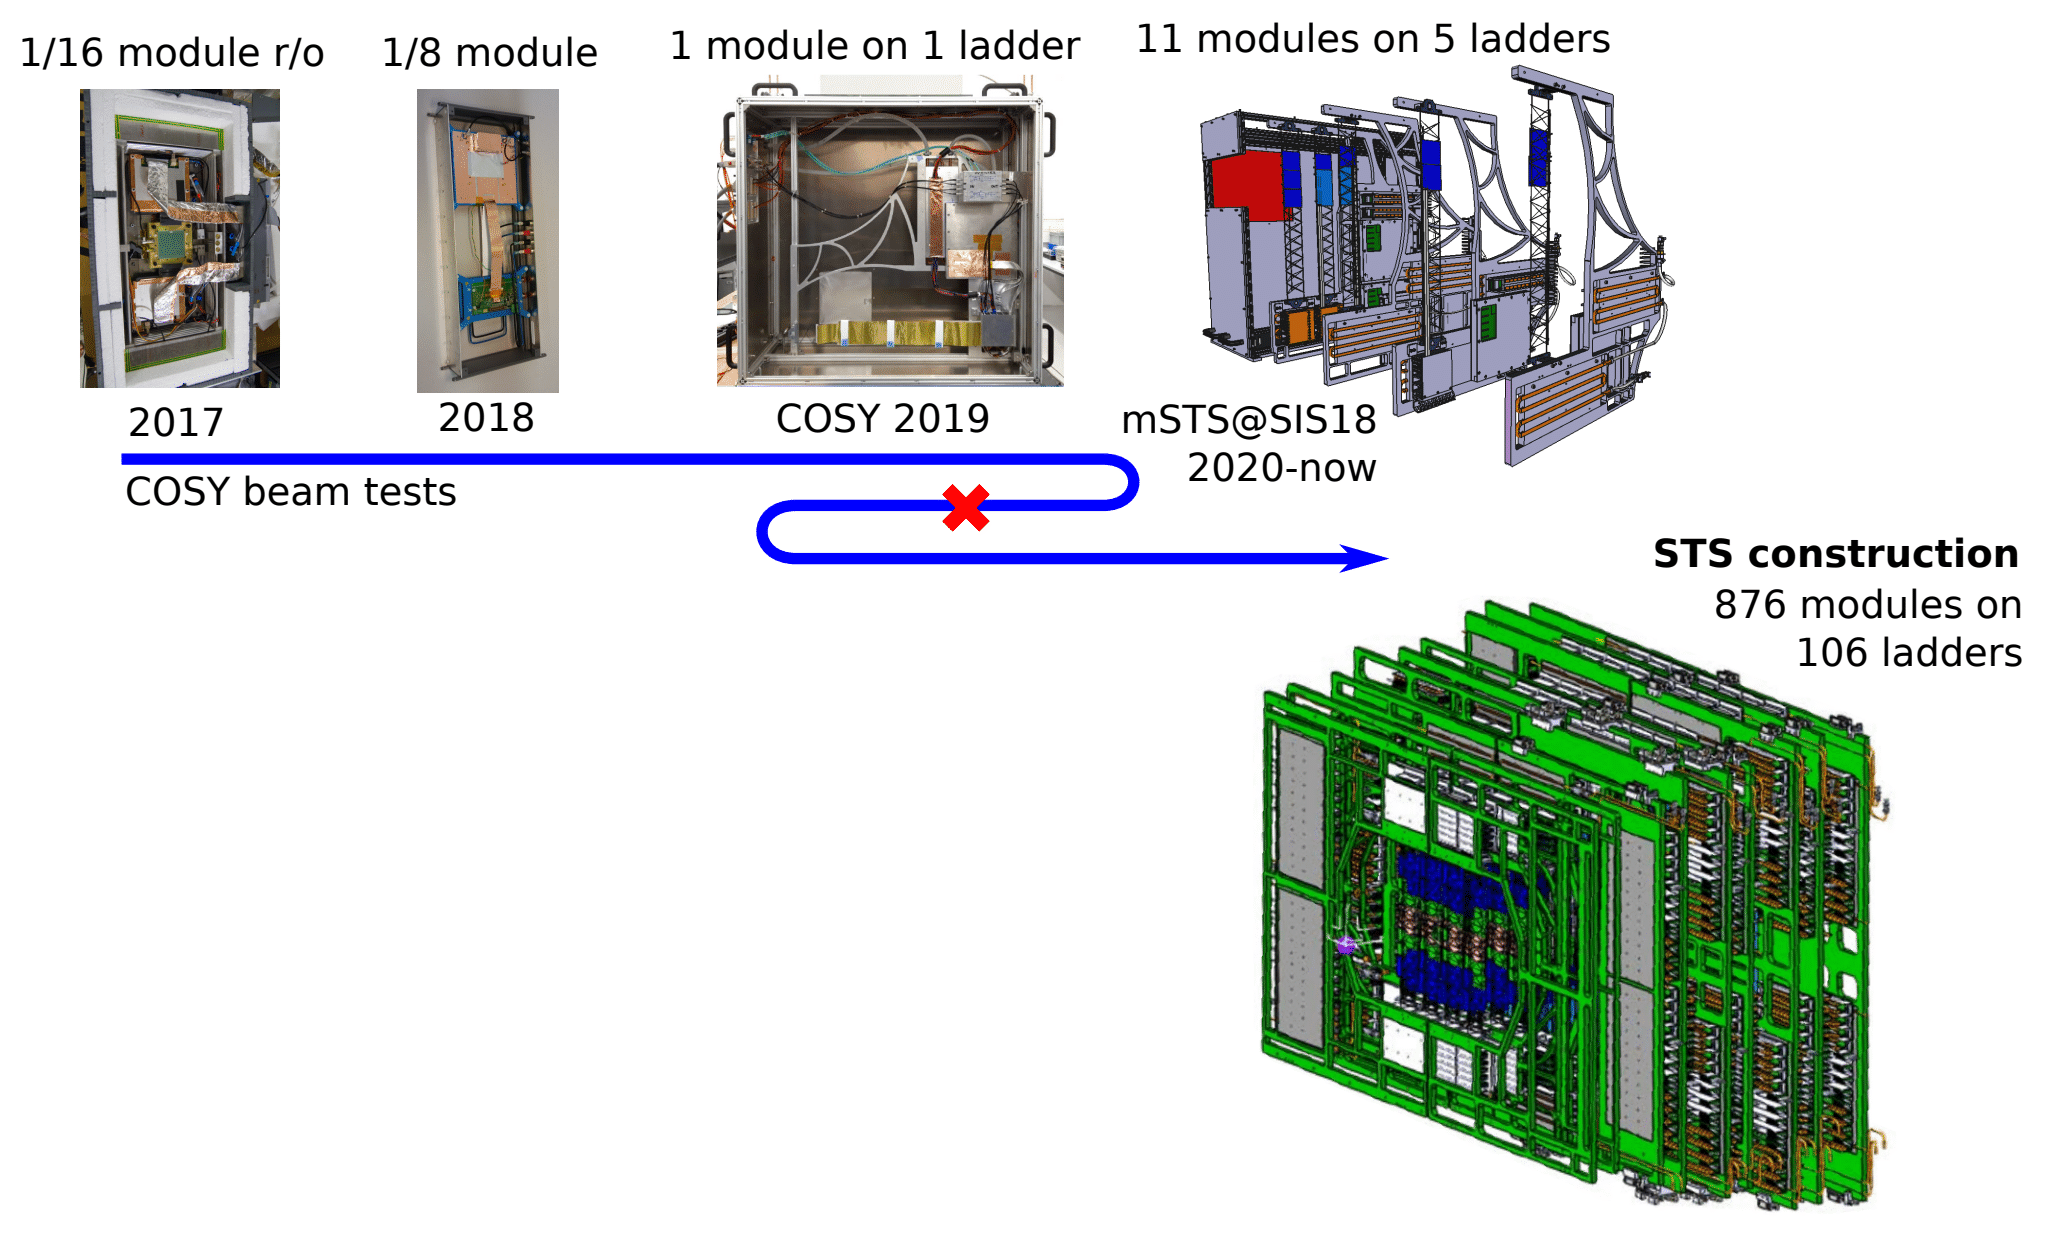
\includegraphics[width=0.95\columnwidth]{Chapter2/images/evolution_sts_new.png}
%\caption{Evolution of the test setups towards \gls{STS}. (Private information %from M. Teklishyn)}
%\label{fig_evolution_STS}
%\end{figure}




\subsection{Double-sided microstrip silicon sensors}
\label{sensors}

The use of microstrip silicon sensors has been demonstrated in many well-known experiments like those operated at \gls{CERN} (\gls{ALICE} and \gls{CMS}) and Brookhaven National Laboratory (\gls{STAR}). The \gls{STS} sensors are produced on \SI{320}{\micro\metre} thick n-type wafers by Hamamatsu Photonics K.K. The $p^{+}$ strips are located on one of the sides (called p-side) forming a pn-junction. The strips at the n-side are isolated using a p-spray technology~\cite{Heuser:54798}. Each of the sensors features 1024 strips with \SI{58}{\micro\metre} pitch. The signal from the sensors is transported to the front-end electronics via ultra-light microcables. These cables are electrically shielded to protect the analog signals from any interference. 

\begin{figure}[!h]
\centering
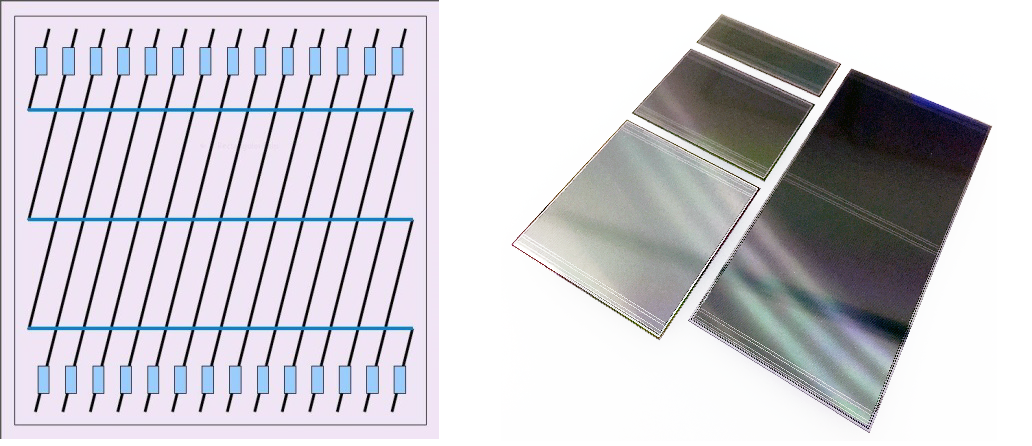
\includegraphics[width=0.75\columnwidth]{Chapter2/images/silicon_sensors.png}
\caption{Left: An example of a sensor electrode segmented into strips inclined by a small angle. The shortest strips are interconnected with each other. Right: The silicon sensors to be used for the \gls{STS}. The width of the sensor is \SI{6.2}{\centi\metre} and there are 4 strip lengths: \SI{2.2}{\centi\metre}, \SI{4.2}{\centi\metre}, \SI{6.2}{\centi\metre}, \SI{12.4}{\centi\metre}~\cite{Heuser:54798}.}
\label{fig_sts_si}
\end{figure}

The aluminum strips on the p-side of the sensors are inclined by \SI{7.5}{\degree} with respect to the n-side. That implies that there is a set of shorter strips on the p-side. These strips are interconnected with each other using a second metallization layer on the sensors. An example of this solution is presented in Figure~\ref{fig_sts_si}. Moreover, to protect the electronics from the dark current, the sensor is AC coupled with the readout.
\subsection{Functional module}
\label{sts_module}
The silicon sensor, the microcables together with the two \glspl{FEB} form a functional module of the \gls{STS}. The assembly is realized stepwise, where each step requires extensive testing of the components. Therefore, a laborious workflow was developed to address the complexity of the module assembly~\cite{carmen2}. 

A module \glspl{ASIC} are powered using low-voltage supply lines. A high voltage supply for the silicon sensor biasing is realized using two separated coaxial lines for positive and negative voltage. The low-voltage powering is provided by dedicated power boards (\gls{POB}), which reside outside the detector acceptance. The \glspl{POB} are populated with DC-DC converters~\cite{DC_DC_converter} which provide the powering for \gls{FEE}. There are two flavors of the DC-DC converters used: 3\,V and 2.5\,V. As the voltage conversion efficiency is not 100\%, the heat produced in this process has to be evacuated. Hence, the \glspl{POB} are in thermal contact with the cooling plates. 

Upon completion of calibration and testing, the module together with the cooling fin is installed onto a carbon-fiber support structure (ladder). Up to ten modules form one carbon ladder. Subsequently, the ladders are mounted on a C-frame, which accommodates a cooling structure. 
\section{The readout chain of the STS}
\label{readout}
\label{DAQ}
The \gls{STS} readout chain is designed to control, readout, and preprocess analog signals acquired from the silicon sensors. The \gls{CBM} experiment is going to run with a free-streaming Data Acquisition (\gls{DAQ}) system. Moreover, it has to handle a high data throughput and store it. It consists of the \gls{FEE}, data transport, online event reconstruction, and online event selection~\cite{Kasinski1}.

The first layer of the \gls{STS} readout chain is a Front-End Board (\gls{FEB}) which is populated with eight Application-Specific Integrated Circuits (ASICs)~\cite{Kasinski2}. Each STS-XYTER \gls{ASIC} is responsible for the readout of 128 channels. The chips feature the analog front-end (\gls{AFE}), generation of hits using an Analog Digital Converter (\gls{ADC}), and timestamp information. 

The next element is the readout board (\gls{ROB}). It aggregates data from multiple \glspl{FEB} and sends it via optical links out of the detector enclosure to the Common Readout Interface (\gls{CRI}) board. Subsequently, the data is transported to a computing farm for online processing, the First Event Level Selector (\gls{FLES}). 

In total, the \gls{STS} features roughly, 14000 STS-XYTERs, 600 \glspl{ROB}. It requires not only extensive testing capabilities but also the possibility to handle a high data throughput. Given a typical average raw event size of roughly 50\,kB for minimum-bias Au+Au collisions, a peak collision rate of 10\,MHz results in an instantaneous raw data rate of about 500\,GB/s (for all the detector systems). Figure~\ref{fig_daq_schem} depicts the complete readout chain of the \gls{STS} at the \gls{CBM} experiment. 

\begin{figure}[!h]
\centering
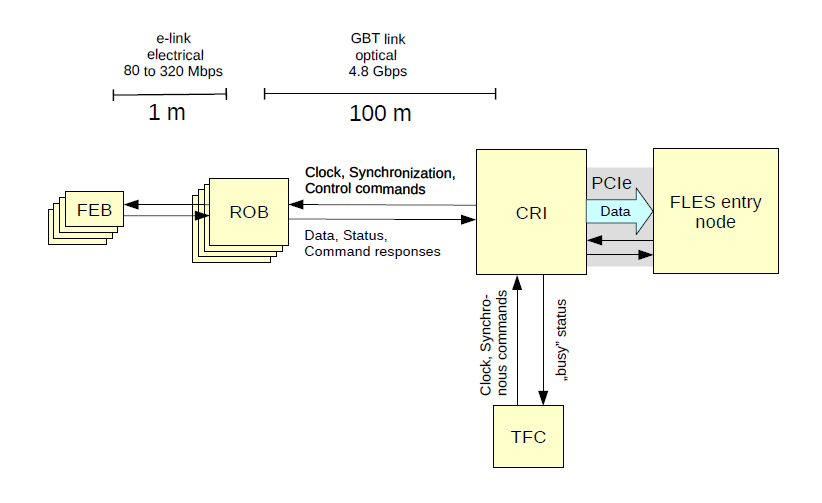
\includegraphics[width=0.8\columnwidth]{Chapter2/images/CRI_DAQ.png}
\caption{The basic building parts for one \gls{FLES} entry node are shown schematically. An entry node can hold multiple \glspl{CRI}. A \gls{CRI} serves up to 8 or 12 \glspl{ROB}, whereas a \gls{ROB} can serve up to \glspl{FEB}. The Timing and Fast Control (\gls{TFC}) is a core system that is shared by all \glspl{CRI}.}
\label{fig_daq_schem}
\end{figure}

There are two other readout chains that have been exercised for different detector development activities. The first option uses on Data Processing Board (\gls{DPB}), a precursor
to the CRI-based readout. The second option is based on the GBTxEMU-based tester, which emulates the \gls{ROB}.


\subsection{Front-end electronics and the readout ASIC}

A readout of a detector module is based on the two \glspl{FEB} (see Figure~\ref{fig_feb}) which have 8 STS-XYTERs each. These chips discriminate and digitize the analog signals coming through the microcables from the silicon strips. As described in the section \ref{STS}, the \glspl{FEB} are located in the perimeter of the detector stations and will receive up to 100\,krad/year~\cite{Heuser:54798}.

\begin{figure}[!h]
\centering
\includegraphics[width=0.45\columnwidth]{Chapter2/images/feb_8_v2.pdf}
\caption{Prototype design of a \gls{FEB} for reading out 1024 channels from a silicon sensor. There are 8 readout ASICs and four low dropout voltage regulators on the left. These active parts are covered by a protective glue called glob top.}
\label{fig_feb}
\end{figure}

The data load for the sensors will vary depending on their position in the detector. Each readout link of the \gls{FEB} has a bandwidth of about 320 Mb/s, therefore for the innermost sensors the \gls{FEB} has 5 readout links instead of 2 or 1. 

The dimensions of the \gls{FEB} are tightly constrained due to the limited space inside the \gls{STS}. Hence, the dimensions of the \gls{FEB} are approximately \SI{3}{\centi\metre} by \SI{10}{\centi\metre}. The chips need also to be powered, which is achieved by the onboard linear voltage regulators (\gls{LDO} regulators). Each \gls{ASIC} has an analog (VDDM) and digital power domain that are powered by 1.2\,V and 1.8\,V \glspl{LDO}. The analog part is powered by 1.2\,V and 1.8\,V \glspl{LDO}, whereas the digital part is supplied from 1.8\,V \gls{LDO}.

\glspl{FEB} are glued to aluminum fins, in order to achieve good thermal coupling. Subsequently, the fins are fixed to the base plate of the \gls{FEB} box (see Figure~\ref{feb_box}) before mounting them on a ladder. The \gls{FEB} boxes reside on cooling plates. The carbon composite, which is the interface between the fin and base plate, has an ultrahigh thermal conductivity. Therefore, the excess heat is efficiently removed by the coolant (NOVEC 649) which circulates through the cooling plate providing temperature down to \SI{-40}{\celsius}. 

\begin{figure}[!h]
\centering
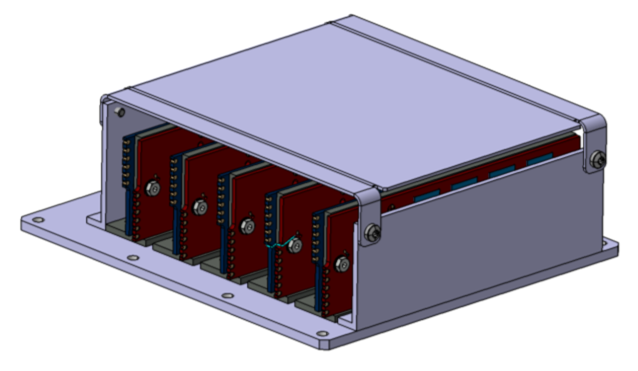
\includegraphics[width=0.55\columnwidth]{Chapter2/images/feb_box_1.png}
\caption{A simplified CAD drawing of the \gls{FEB} box.}
\label{feb_box}
\end{figure}


The characterization of the STS-XYTER ASICs is an extensive procedure that investigates the chip. Information about proper amplitude and time calibrations is necessary to interpret the data correctly. This represents an essential step before using the chip in the readout of the silicon sensors. The characterization procedures are intended to
check many parameters that influence the \gls{FEB} performance. 


\subsubsection{Design of the STS-XYTER}

The STS-XYTER (see Figure~\ref{sts_xyter}) is an integrated circuit designed for the readout of \gls{STS} and \gls{MUCH} consisting of 128 analog channels. One of the elements of the chip is a so-called low noise Charge Sensitive Amplifier (\gls{CSA}), which converts the collected charge into a voltage signal with an amplitude proportional to the charge. Subsequently, the signals pass through the Polarity Selection Circuit (\gls{PSC}) which allows measuring both polarities
  of the detector signal with the same \gls{ASIC}. It makes the use of the \gls{ASIC} for double-sided silicon sensors feasible. Signal processing is distinguished into two paths: fast and slow. The first one is responsible for the determination of the timestamp and the second one has been adjusted for low noise discrimination and energy measurement with a 5-bit flash \gls{ADC}. When operating the \gls{ASIC} in self-triggered mode, hit information is saved and latched by the arrival of each signal using the information from the 5-bit continuous-time \gls{ADC} and the slow path. 

\begin{figure}[!h]
\centering
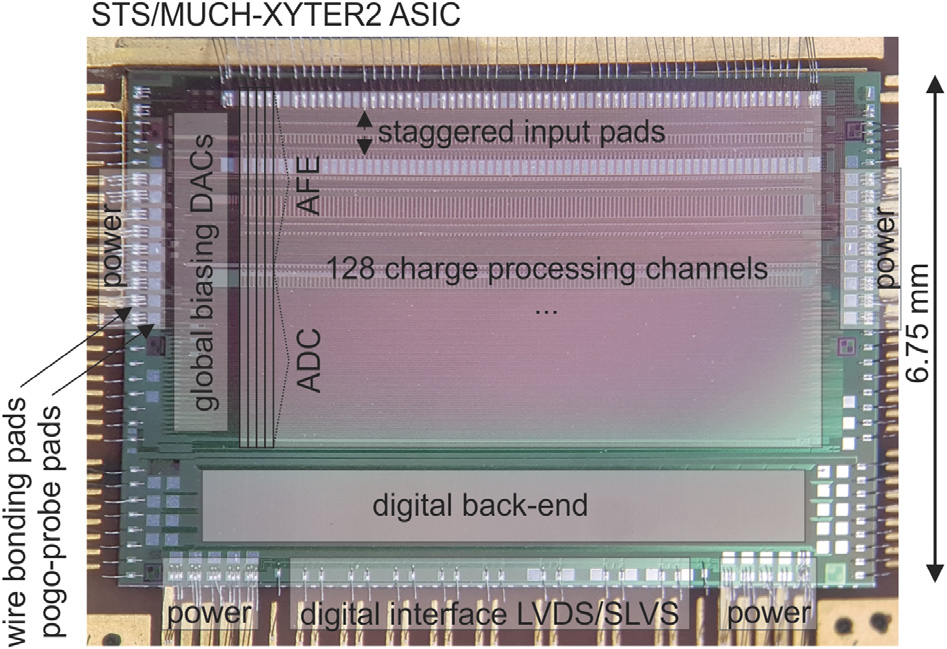
\includegraphics[width=0.65\columnwidth]{Chapter2/images/ASIC2.2.png}
\caption{The final version of the STS-XYTER chip with the major parts marked~\cite{KASINSKI2018225}.}
\label{sts_xyter}
\end{figure}

The digital back-end allows accessing registers and readout the data. It also provides measures to monitor the performance of the chip via i.e., upset counters, link error monitor, and diagnostic circuitry (temperature, VDDM potential, CSA bias value). The serial communication with the chip is based on a custom-developed Hit and Control Transfer Synchronous Protocol (STS-HCTSP) protocol~\cite{Kasinski_2016}. A detailed description of the STS-XYTER can be found in~\cite{RodriguezRodriguez2020}.

STS-XYTER also features an internal monitoring circuit - a diagnostic circuit. It enables the measurement of several potentials inside the chip. By monitoring the analog powering domain (VDDM), temperature, it is possible to have a general understanding of the chip state without running extensive tests. The diagnostic circuit of the \glspl{ASIC} and the obtained results will be discussed in detail in Chapter 4.
\subsubsection{Noise considerations for the detector module}
Noise levels are one of the most important parameters for the \gls{STS}. The contribution of noise becomes even more crucial in triggerless systems like the \gls{CBM} experiment. The noise hit is produced once it exceeds the set thresholds of the \gls{ADC} discriminator. It is digitized and constitutes the data together with the real hits. Too high noise levels may not only worsen the obtained data but also affect the performance of the \gls{DAQ} chain~\cite{Heuser:54798}.

The noise level is relatively high due to the fast path higher bandwidth. The slow path, on the other hand, has been adjusted for minimal noise, allowing the hit to be triggered whenever a slow shaper signal passes the ADC first comparator threshold~\cite{RodriguezRodriguez2020}. The noise level may be influenced by a number of factors including load capacitance 
(different silicon sensors sizes and microcable lengths), peaking time, temperature, glob-top type, powering, and external contributions.

In order to estimate the overall noise performance it's necessary to include the silicon sensor, cables, and readout chip. There are three main contributions to the noise levels~\cite{Toia:209729}:
\begin{itemize}
    \item parallel current noise (detector leakage current, leakage current flowing through transistors in the Electrostatic Discharge protection circuit, resistor bias shunt resistance~\cite{Spieler}, feedback resistance),
    \item series white noise (\gls{CSA} input transistor thermal and flicker noise)
    \item series 1/f (flicker) noise (caused by charge carriers that are randomly trapped and released between the interfaces of two materials).
\end{itemize}
An analytical expression of the noise spectral density at the shaper output and the Equivalent Noise Charge (\gls{ENC}) can be expressed as:
\begin{equation}
    ENC^{2} = ENC^{2}_{i} + ENC^{2}_{w} + ENC^{2}_{1/f},
\end{equation}
where $ENC_{i}$  is the total current noise, $ ENC_{w}$ is the total white noise and $ENC_{1/f}$ is the total flicker noise. 

The noise performance of a module provides an invaluable insight into the state of the sensor and \gls{FEE} electronics. Knowing the nominal \gls{ENC} allows the detection and investigation of potential external noise sources. Moreover, it provides means of estimating broken analog connections or hints on how to adjust settings to reduce the noise contribution.
\subsection{Readout board and Common Readout Interface}

The \gls{STS} readout board (\gls{ROB}) is a data concentrator board based on the radiation-tolerant GBTx ASIC and Versatile Link
devices developed by CERN and others~\cite{Bonacini:1235849, C_2013}. The board is an interface between many electrical readout links (many \glspl{FEB}) and the \glspl{CRI} boards located outside the underground cavern of the \gls{CBM} experiment~\cite{Lehnert_2017}. It resides inside the \gls{STS} enclosure, which means that it will be exposed to high levels of ionizing particles. Therefore, it is built from radiation hard components. The board is also thermally coupled to the cooling plate, which can reach a temperature down to \SI{-40}{\degree}. The \gls{ROB} needs to reliably work at changing temperature between \SI{-40}{\degree} and \SI{20}{\degree}. 

The main building elements of the board are three \gls{GBT}x \glspl{ASIC} and a \gls{GBT} \gls{SCA2} \gls{ASIC}. Two of the \glspl{GBT}x \glspl{ASIC} act as slaves and are controlled via the mentioned \gls{SCA2}. 

The Common Readout Interface (\gls{CRI}) is a PCIe card\footnote{PCIe card refers to a kind of network adapter with a PCIe interface.} based on Field Programmable Gate Arrays (\gls{FPGA}). The \gls{CRI} provides the input to the First-level Event Selector (\gls{FLES}). It is also a central element of the \gls{DAQ} chain, as it provides means of data control. Moreover, the \gls{CRI} has an interface to the \gls{TFC} system. 
\begin{figure}[!h]
\centering
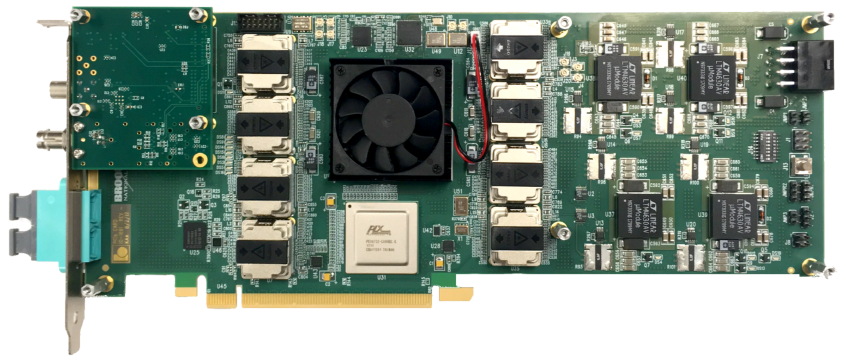
\includegraphics[width=0.8\columnwidth]{Chapter2/images/cri_board_atlas.pdf}
\caption{The first prototype of the \gls{CRI} board~\cite{CRI}.}
\label{fig_cri_board}
\end{figure}


\subsection{Alternative readout chains}
\label{tester}
There are two alternative readout chains implemented for testing purposes towards the realization of \gls{STS}. The first readout chain is based on the Data Processing Board (\gls{DPB} is a \gls{FPGA} based board), \glspl{ROB}. The second type of readout chain is GBTxEMU-based. It is an alternative low-cost readout chain that can be used for
low-performance setups, e.g., for testing and quality assurance. \bigbreak


\textbf{DBP based chain}\bigbreak


Even though the final solution for the readout is the \gls{CRI} board, the Data Processing Boards (\glspl{DPB}) were implemented for developing and testing purposes~\cite{Loizeau}. For the control communication with the \gls{DPB}, the IPbus protocol~\cite{ipbus} was chosen. It is a communication protocol based on Gigabit Ethernet (GbE) which allows simple and fast communication with \glspl{FPGA}.

\textbf{GBTxEMU} \bigbreak


Another alternative to the two readout chains is the GBTxEMU-based tester. It is based on a commercial Artix-7 board (TE-0712, Trenz Electronics Gmbh), and allows emulating GBTX ASIC or the whole \gls{ROB}. Moreover, it could also be used in an autonomous mode with the addition of an adapter.


The whole examination process towards \gls{STS} will include testing of about 20000 ASICs, then 2000 FEBs (tested  multiple times during the assembly, e.g., after the ASIC wire bonding and after the micro-cable bonding), and eventually the full module. As a hardware platform offering good availability and reasonable production cost, the GBTx65 EMU~\cite{zabolotny1} board was chosen.

The software used for the operation of the emulator board is also based on the IPbus~\cite{ipbus} protocol to access registers.
The operation begins with the full synchronization of the STS-XYTER links. This process enables communication with the chip, given no correct time phase between data and clock and incoming data exists. The next step involves the configuration of the chip registers (35496 bits for the AFE control are set). At the same time, the number of enabled up-links, the channel masking, and the timestamp counter are set.  From this point on, any custom tests or calibration may proceed. For example, read and write register tests, readout of the VDDM potential values, chip temperature, etc. Moreover, to enable long-term testing, an interface to the control system framework was implemented.

\section{Highlights from the performance simulations of the STS}
The STS performance is mainly determined by its ability to accurately reconstruct tracks of charged particles, which can then be used to determine the momentum of those particles accurately. During the \gls{CBM} experiment, silicon sensors will be exposed to a total fluence of up to $10^{14}\,\mathrm{n_{eq}cm^{-2}}$ which causes a decrease of Charge Collection Efficiency (CCE) (Figure~\ref{fig_cce}) and enhanced noise. 

\begin{figure}[!h]
\centering
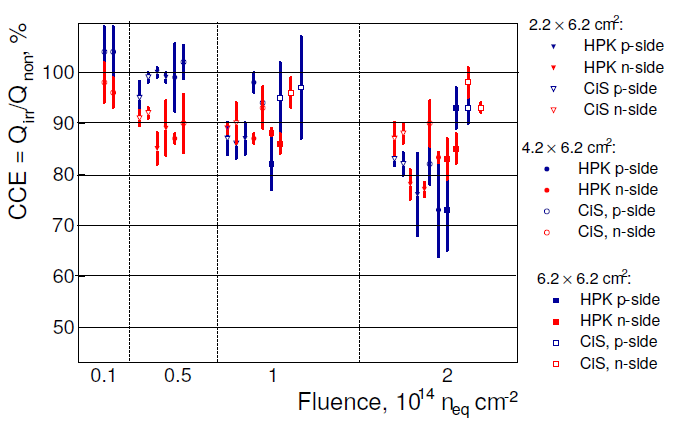
\includegraphics[width=0.8\columnwidth]{Chapter2/images/CCE.png}
\caption{CCE as a function of the fluence for sensors studied during the prototyping phase for \gls{STS}. To ensure the full depletion the sensors were biased to 450\,V for fluences up to $1\times10^14\mathrm{MeV n_{eq}cm^{-2}}$. For the highest fluence the bias voltage was 500\,V~\cite{Momot:2019lnx}.}
\label{fig_cce}
\end{figure}

This problem can be addressed from a few different perspectives. Firstly, the noise levels of the newly produced modules should be as low as possible. It can be achieved using low-noise electronics and ensuring proper shielding from electromagnetic interference. The noise levels can also be adjusted by decreasing the temperature or annealing the sensors. Nevertheless, the latter has to be performed in a controlled fashion in order to avoid reverse annealing. Keeping the detectors at temperatures below \SI{0}{\celsius} eliminates the reverse term while largely preserving the beneficial one. During maintenance, the ambient temperature has to be raised in a controlled manner to take advantage of short-term annealing and to prevent any reverse effects~\cite{Hartmann:2017gzy}. Figure~\ref{fig_cce_temp} shows how the silicon sensor would behave after receiving up to $10\times10^{13}\,\mathrm{MeV n_{eq}cm^{-2}}$, what is considered to be the maximum dose that the \gls{STS} sensors will receive. According to this plot, the assumed signal-to-noise ratio of 10 can be achieved even if the sensor \gls{CCE} drops to 70\% if the temperature is kept at \SI{-10}{\celsius}.

\begin{figure}[!h]
\centering
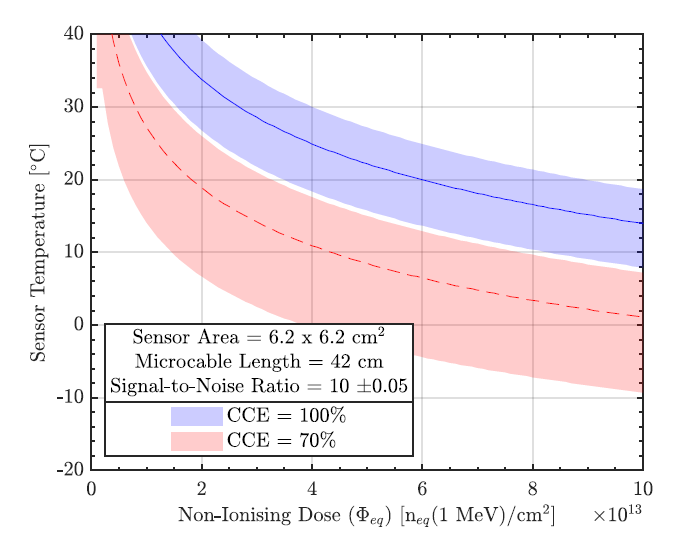
\includegraphics[width=0.7\columnwidth]{Chapter2/images/SN.png}
\caption{Variation of the sensor temperature with accumulated fluence to maintain S/N = 10 for two different CCE levels. The shaded bands indicate 20\% modeling error~\cite{Agarwal}.}
\label{fig_cce_temp}
\end{figure}

%\bigbreak
%\textbf{Track reconstruction efficiency and momentum resolution}

%Except for the case of neutral charged particles, STS takes part in the registration of almost all CBM observables.
%The track finding in STS, operated in an inhomogeneous magnetic field, is based on the Cellular Automaton method [77, 78]. A dedicated software package based on the Kalman filter [79] procedure is %used for track fitting and reconstruction of primary and secondary vertices with the precision
%allowed by the granularity of the detector.

\section{Overview of the services for the STS}

The \gls{STS} will feature a number of services and sensors that need to be controlled, monitored, and automatized in order to work efficiently during the operation of the detector. The data from these services provides unique information about the detector state and functioning:
\begin{enumerate}
    \item Low voltage and high voltage powering modules.\\
    About 2500 low voltage and 1800 high voltage powering channels will be employed for the \gls{STS}. The low-voltage modules will be located in the experiment cave. This location exposes the electronics to elevated radiation levels. 
    \item Temperature, humidity, pressure sensors.\\
    A number of different sensors and technologies will be used to monitor the ambient conditions inside the detector. Their performance and values are going to have a direct impact on the detector operation.
    \item Cooling plant.\\
    To avoid reverse annealing of the silicon sensors and thermal runaway scenarios, the detectors will be cooled with temperatures reaching \SI{-40}{\degree} at the end of their lifetime. The cooling plant providing the coolant is a crucial part of the safe operation of the detector.
    \item Air-drying system.\\
    The coldest points inside the \gls{STS} may reach temperatures down to \SI{-40}{\degree}. Therefore, the frost point inside the enclosure has to be fairly below the coolant temperature to avoid possible icing or condensation on the electronics.
 \end{enumerate}

%\subsection{Powering schematics of the detector}
%\label{powering}
%\subsection{Cooling concept for the STS's electronics and %silicon sensors}
%\label{cooling}


\section{Requirements for the control system}
\label{sys:req}
Custom solutions that are applied to \gls{STS} make the control of this system very challenging. Different services imply different control solutions which need to be implemented.
A distributed control system should offer remote control, alarm detection, reporting and logging, data processing (archiving, retrieval, plotting, conversion, analysis), common time management, access security, and automatic sequencing\footnote{Sequencing, also known as sequential control, it controls the device in a pre-determined order.}.
In addition to that, the \gls{DCS} for the Silicon Tracking System (\gls{STS}) is being designed taking into consideration the following aspects:

 
 \begin{itemize}
    \item potential control framework should offer the possibility to control a variety of different services, which often have different communication protocols,
    \item logging, and monitoring - there should be reliable means of supervision of processes, containers, and Input/Output Controllers\footnote{The input/output controller is a device that interfaces between an input or output device and the computer or hardware device} (\glspl{IOC}).
    \item the control software should be horizontally and vertically scalable, when it comes to adding additional computing nodes or applications/Input Output Controllers (\glspl{IOC})/containers,
    \item supervision - it should be possible to integrate a sub-system oriented with higher-level control structures,
     \item flexible - applications should be easy to run on different operating systems and processor architectures,
     \item sustainability and support - the experiment is supposed to run for about 10 years, excluding the building and commissioning time. The control system should be sustainable and long-term support provided,
     \item reliability - the system should be highly available, minimizing the downtimes,
     \item network separation - it should be running in a dedicated network (divided into several service-oriented subnets) to have a good overview of the processes and communication between the nodes,
     \item \glspl{GUI} - all parameters/process variables\footnote{In control theory, a process variable is the currently measured value of a particular part of a process which is being monitored or controlled} should be available in a user-friendly Graphical User Interface (\gls{GUI}). In case of error or malfunction, it should be stated clearly by the software where the error happened, what could be the potential risk, and what actions need to be taken.

 \end{itemize}
\newpage

